\documentclass[11pt,a4paper]{article}

\usepackage[utf8]{inputenc}
\usepackage[T1]{fontenc}
\usepackage{geometry}
\geometry{margin=2.5cm}
\usepackage{listings}
\usepackage{xcolor}
\usepackage{hyperref}
\usepackage{enumitem}
\usepackage{booktabs}
\usepackage{tabularx}
\usepackage{parskip}
\usepackage{titlesec}
\usepackage{tikz}
\usetikzlibrary{arrows.meta, positioning, fit, calc}
\newcolumntype{Y}{>{\raggedright\arraybackslash}X}

\hypersetup{colorlinks=true, linkcolor=blue!50!black, urlcolor=blue!50!black, citecolor=blue!50!black}

\definecolor{codebg}{RGB}{245,245,245}
\definecolor{codegray}{RGB}{110,110,110}
\definecolor{codegreen}{RGB}{0,110,0}
\definecolor{codeblue}{RGB}{30,80,180}

\lstdefinestyle{code}{
    backgroundcolor=\color{codebg}, basicstyle=\ttfamily\footnotesize,
    keywordstyle=\color{codeblue}, commentstyle=\color{codegray}\itshape,
    stringstyle=\color{codegreen}, breaklines=true, breakatwhitespace=false,
    frame=single, rulecolor=\color{black!15}, numbers=left,
    numberstyle=\tiny\color{codegray}, xleftmargin=1.8em, framexleftmargin=1.5em,
    showstringspaces=false, tabsize=2,
    literate=
      {á}{{\'a}}1 {à}{{\`a}}1 {ã}{{\~a}}1 {â}{{\^a}}1
      {é}{{\'e}}1 {ê}{{\^e}}1 {í}{{\'i}}1
      {ó}{{\'o}}1 {õ}{{\~o}}1 {ô}{{\^o}}1 {ú}{{\'u}}1
      {ç}{{\c c}}1 {Á}{{\'A}}1 {É}{{\'E}}1 {Í}{{\'I}}1
      {Ó}{{\'O}}1 {Ú}{{\'U}}1 {Ã}{{\~A}}1 {Õ}{{\~O}}1
      {Ç}{{\c C}}1 {°}{{\textdegree}}1,
}
\lstset{style=code}

\titleformat{\section}{\normalfont\Large\bfseries}{\thesection}{1em}{}
\titleformat{\subsection}{\normalfont\large\bfseries}{\thesubsection}{1em}{}

\sloppy

% Estilos dos diagramas
\tikzset{
    blk/.style={draw=black!60, fill=blue!5, rounded corners=2pt, align=center,
                font=\footnotesize, minimum height=1.05cm, text width=2.5cm, inner sep=3pt},
    fut/.style={draw=black!45, dashed, fill=black!3, rounded corners=2pt, align=center,
                font=\footnotesize, minimum height=1.05cm, text width=2.5cm, inner sep=3pt},
    arr/.style={-{Latex[length=2mm]}, thick, black!70},
    farr/.style={-{Latex[length=2mm]}, thick, black!45, dashed},
    lab/.style={font=\scriptsize\itshape, text=black!70, align=center},
}

\title{\textbf{TelemetriaMqtt v2 --- Firmware} \\[4pt]
\large Como funciona, o que cada parte faz e em que estado está}
\author{Projeto de Telemetria FSAE}
\date{18 de setembro de 2026}

\begin{document}
\maketitle

\begin{abstract}
\noindent Este documento explica o firmware do ESP32 do projeto: qual é o seu papel no sistema, como o código está organizado, o que acontece do momento em que um quadro CAN chega ao fio até o valor de um sinal ficar disponível na memória, e como se testa cada parte. O firmware está \textbf{parcialmente implementado}: leitura e decodificação do CAN existem e são testadas (checkpoint 8); WiFi, MQTT e TLS ainda não (checkpoint 9). O documento separa com clareza o que já existe do que ainda é plano.
\end{abstract}

\tableofcontents

\section{Papel do firmware no sistema}

O carro tem um módulo de distribuição de energia, o \textbf{PDM32} (AIM), que já mede as correntes das cargas, a tensão da bateria e outros sinais do motor. Ele transmite esses valores continuamente no barramento \textbf{CAN2} a 500~kbps, em 10 quadros diferentes (IDs \texttt{0x100} a \texttt{0x131}) configurados no software Race Studio.

O firmware roda num \textbf{ESP32} e tem uma única missão: \emph{ouvir esse barramento, entender os quadros e transformá-los nos 20 sinais de telemetria}, para que sejam enviados por MQTT ao resto do sistema (broker, ingestão, InfluxDB, Grafana). O ESP32 não mede nada por conta própria e não comanda nada no carro; ele só observa e repassa.

\begin{figure}[h]
\centering
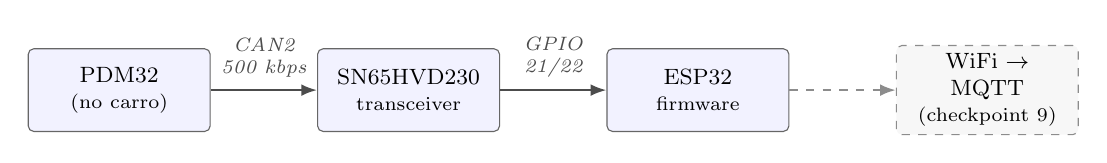
\begin{tikzpicture}[node distance=1.35cm, blk/.append style={text width=2.1cm}, fut/.append style={text width=2.1cm}]
    \node[blk] (pdm) {PDM32\\ \scriptsize (no carro)};
    \node[blk, right=of pdm] (xcvr) {SN65HVD230\\ \scriptsize transceiver};
    \node[blk, right=of xcvr] (esp) {ESP32\\ \scriptsize firmware};
    \node[fut, right=of esp] (mqtt) {WiFi $\to$ MQTT\\ \scriptsize (checkpoint 9)};
    \draw[arr] (pdm) -- node[lab, above=1pt] {CAN2\\500 kbps} (xcvr);
    \draw[arr] (xcvr) -- node[lab, above=1pt] {GPIO\\21/22} (esp);
    \draw[farr] (esp) -- (mqtt);
\end{tikzpicture}
\caption{Cadeia física. As caixas tracejadas ainda não existem.}
\end{figure}

\subsection{Por que um transceiver externo}

O ESP32 tem o \emph{controlador} CAN embutido (chamado \textbf{TWAI}, \emph{Two-Wire Automotive Interface}, compatível com CAN 2.0), mas não tem o \emph{transceiver}, o circuito que converte os níveis lógicos de 3,3~V nos níveis diferenciais do barramento. Por isso existe o SN65HVD230, que opera a 3,3~V e liga direto nos GPIOs do ESP32, sem conversor de nível.

\section{Estado atual: o que existe e o que falta}

\begin{center}
\begin{tabularx}{\textwidth}{lYl}
\toprule
\textbf{Função} & \textbf{Situação} & \textbf{Checkpoint} \\
\midrule
Ler quadros do CAN2 pelo TWAI (500 kbps) & Implementado, compila; \emph{não testado com hardware} & 8 \\
Decodificar os 10 payloads nos 20 sinais & Implementado e testado (20 testes nativos) & 8 \\
Imprimir resumo na serial para conferência & Implementado & 8 \\
Conectar ao WiFi & Não implementado & 9 \\
Montar o JSON e publicar por MQTT & Não implementado & 9 \\
TLS com certificado do broker & Não implementado & 9 \\
Validação com hardware e com o carro & Depende de o hardware chegar & 11 \\
\bottomrule
\end{tabularx}
\end{center}

Em termos práticos: hoje o firmware, ligado a um barramento CAN real, faria o ESP32 receber e decodificar os quadros e mostrar na serial um resumo a cada segundo. Nada sai do ESP32 pela rede. O arquivo \texttt{include/secrets.h.example} (credenciais de WiFi e MQTT) já existe como modelo, mas nenhum código o usa ainda.

\section{Estrutura do projeto}

\begin{lstlisting}[caption={Árvore de firmware/ (sem arquivos gerados)}]
firmware/
  platformio.ini              dois ambientes: esp32dev e native
  include/
    secrets.h.example         modelo de credenciais (ainda não usado)
  lib/can_parser/
    can_parser.h              CanFrame, Telemetry, parse_frame()
    can_parser.cpp            decodificação (C++17 puro)
  src/
    main.cpp                  setup() / loop() do ESP32
    can_twai.h / can_twai.cpp driver TWAI (só esp32dev)
  test/
    test_scaffolding/         prova de que o harness de testes roda
    test_can_parser/          20 testes do parser
\end{lstlisting}

\subsection{Dois ambientes de compilação}

O \texttt{platformio.ini} define dois ambientes com propósitos diferentes:

\begin{center}
\begin{tabularx}{\textwidth}{llX}
\toprule
\textbf{Ambiente} & \textbf{Plataforma} & \textbf{Para que serve} \\
\midrule
\texttt{esp32dev} & ESP32 (framework Arduino) & Gera o firmware de verdade. Compila \texttt{src/} e \texttt{lib/}. Gravar exige o ESP32 conectado por USB. \\
\texttt{native} & PC (Linux) & Roda os testes unitários com o framework Unity, sem hardware. Compila só \texttt{lib/} e \texttt{test/}. \\
\bottomrule
\end{tabularx}
\end{center}

A divisão do código segue essa separação. Tudo o que tem \emph{lógica} (a decodificação) fica em \texttt{lib/can\_parser}, sem nenhuma dependência de Arduino ou ESP-IDF, e por isso compila nos dois ambientes. Tudo o que depende do chip (o driver TWAI, \texttt{Serial}, \texttt{millis()}) fica em \texttt{src/}, que só existe no \texttt{esp32dev}.

\section{Como o firmware funciona}

\subsection{Visão do fluxo de dados}

\begin{figure}[h]
\centering
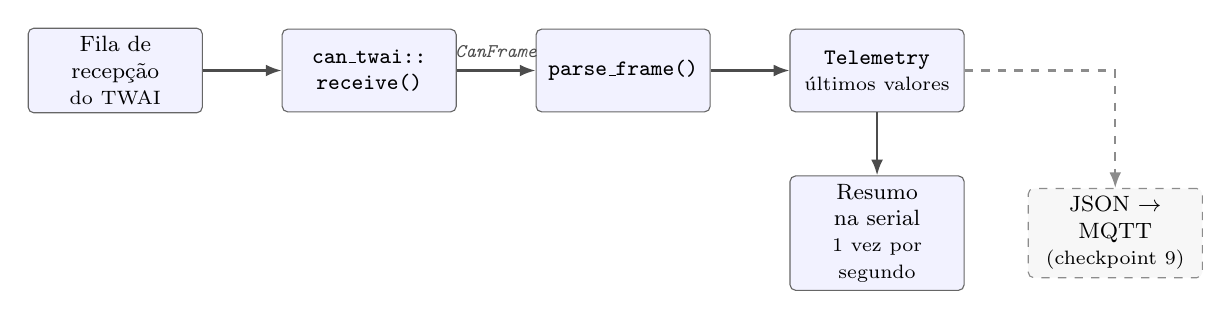
\begin{tikzpicture}[node distance=1.0cm, blk/.append style={text width=2.0cm}, fut/.append style={text width=2.0cm}]
    \node[blk] (fila) {Fila de recepção\\ \scriptsize do TWAI};
    \node[blk, right=of fila] (recv) {\texttt{can\_twai::}\\\texttt{receive()}};
    \node[blk, right=of recv] (parse) {\texttt{parse\_frame()}};
    \node[blk, right=of parse] (tel) {\texttt{Telemetry}\\ \scriptsize últimos valores};
    \draw[arr] (fila) -- (recv);
    \draw[arr] (recv) -- node[lab, above=1pt] {\texttt{CanFrame}} (parse);
    \draw[arr] (parse) -- (tel);
    \node[blk, below=0.8cm of tel] (ser) {Resumo na serial\\ \scriptsize 1 vez por segundo};
    \node[fut, right=0.8cm of ser] (json) {JSON $\to$ MQTT\\ \scriptsize (checkpoint 9)};
    \draw[arr] (tel) -- (ser);
    \draw[farr] (tel.east) -| (json.north);
\end{tikzpicture}
\caption{Caminho de um quadro dentro do firmware.}
\end{figure}

Os quatro blocos de cima acontecem o tempo todo, dentro do \texttt{loop()}. A leitura para a serial acontece uma vez por segundo. O envio por MQTT é o que falta.

\subsection{Inicialização: \texttt{setup()}}

\texttt{setup()} roda uma vez ao ligar o ESP32 e faz só duas coisas:

\begin{enumerate}
    \item Abre a serial a 115\,200 baud e imprime o nome do firmware.
    \item Chama \texttt{can\_twai::begin()}, que instala e liga o driver CAN. Se falhar, imprime \texttt{TWAI: falha ao iniciar o driver CAN}.
\end{enumerate}

Se o driver não subir, o firmware \textbf{não para}: o \texttt{loop()} continua rodando e a linha de resumo aparece com os contadores em zero. A única pista é a mensagem de erro impressa uma vez no início.

\subsection{Laço principal: \texttt{loop()}}

A cada volta (sem \texttt{delay}, o laço gira o mais rápido possível), o \texttt{loop()} faz:

\begin{enumerate}
    \item \textbf{Esvazia a fila de recepção.} Enquanto \texttt{can\_twai::receive()} devolver um quadro, ele é entregue a \texttt{parse\_frame()}. Se o parser aceitar, incrementa \texttt{frames\_ok}; senão, \texttt{frames\_ignored}.
    \item \textbf{Confere o relógio.} Se passou 1 segundo desde o último relatório, imprime uma linha na serial.
\end{enumerate}

\begin{lstlisting}[language=C++,caption={O coração do main.cpp}]
void loop() {
  can_parser::CanFrame frame;
  while (can_twai::receive(frame)) {
    if (can_parser::parse_frame(frame, telemetry)) {
      frames_ok++;
    } else {
      frames_ignored++;
    }
  }

  const uint32_t now = millis();
  if (now - last_report_ms >= 1000) {
    last_report_ms = now;
    Serial.printf("CAN ok=%lu ignorados=%lu | rpm=%.0f ...\n", ...);
  }
}
\end{lstlisting}

A linha de resumo (formato ilustrativo, não é saída medida) tem este aspecto:

\begin{lstlisting}[caption={Exemplo do formato da linha na serial}]
CAN ok=1980 ignorados=0 | rpm=6500 engineTemp=88.5 extBattery=12.60
\end{lstlisting}

Como ler: \texttt{ok} deve crescer sempre que o PDM estiver transmitindo (o PDM manda cerca de 99 quadros por segundo no total); \texttt{ignorados} deve ficar perto de zero; os três valores acompanham o carro. Diferença de tempo com \texttt{now - last\_report\_ms} usa aritmética sem sinal, então continua correta mesmo quando o contador de milissegundos dá a volta (após cerca de 49 dias ligado).

\section{O protocolo CAN que o firmware entende}

O contrato é a tabela ``Plano de payloads'' do \texttt{SCOPE.md}, que espelha o que foi configurado no Race Studio. Todos os valores são \textbf{little endian}; os \texttt{float} são IEEE 754 de 32 bits.

\begin{center}
\small
\begin{tabularx}{\textwidth}{lrrXX}
\toprule
\textbf{ID} & \textbf{Freq} & \textbf{DLC} & \textbf{Bytes 0--3} & \textbf{Bytes 4--7} \\
\midrule
\texttt{0x100} & 20 Hz & 8 & \texttt{rpm} & \texttt{throttlePosition} \\
\texttt{0x101} & 20 Hz & 8 & \texttt{lambda} & \texttt{map} \\
\texttt{0x110} & 10 Hz & 8 & \texttt{gpsSpeed} & \texttt{shifterCurrent} \\
\texttt{0x111} & 10 Hz & 8 & \texttt{bicosD1Current} & \texttt{bicosD2Current} \\
\texttt{0x112} & 10 Hz & 8 & \texttt{bobinasCurrent} & \texttt{poTotCurrent} \\
\texttt{0x113} & 10 Hz & 8 & \texttt{poTotCrntAll} & \texttt{partidaCurrent} \\
\texttt{0x114} & 10 Hz & 4 & \texttt{extBattery} & --- \\
\texttt{0x120} & 5 Hz & 8 & \texttt{ventoinhaCurrent} & \texttt{bombaCurrent} \\
\texttt{0x130} & 2 Hz & 8 & \texttt{engineTemp} & \texttt{airTemp} \\
\texttt{0x131} & 2 Hz & 8 & \texttt{brakeLightCurrent} & \texttt{bombaInput}, \texttt{giratoriaInput} (\texttt{uint16}, bytes 4--5 e 6--7) \\
\bottomrule
\end{tabularx}
\end{center}

\subsection{Exemplo: um quadro vira dois sinais}

Suponha que chega um quadro com ID \texttt{0x100}, DLC 8 e estes 8 bytes de dados:

\begin{center}
\ttfamily
\begin{tabular}{|c|c|c|c|c|c|c|c|}
\hline
00 & 50 & 9A & 44 & 00 & 00 & 48 & C1 \\
\hline
\multicolumn{4}{|c|}{bytes 0--3} & \multicolumn{4}{c|}{bytes 4--7} \\
\hline
\end{tabular}
\end{center}

O parser separa em duas palavras de 4 bytes e reordena cada uma do little endian para o valor de 32 bits:

\begin{itemize}
    \item bytes \texttt{00 50 9A 44} $\to$ \texttt{0x449A5000} $\to$ \textbf{1234,5} $\to$ \texttt{rpm}
    \item bytes \texttt{00 00 48 C1} $\to$ \texttt{0xC1480000} $\to$ \textbf{$-12{,}5$} $\to$ \texttt{throttlePosition}
\end{itemize}

(Os valores do exemplo foram escolhidos para a conta ficar fácil de acompanhar; não são leituras reais do carro.)

\subsection{Frequências diferentes, um único estado}

Os payloads chegam em ritmos distintos (20, 10, 5 e 2 Hz). Por isso o firmware não guarda ``o último quadro'', e sim os \textbf{últimos valores conhecidos de cada sinal}. Cada quadro atualiza apenas os campos do seu ID e deixa os outros como estavam. A estrutura que faz isso é a \texttt{Telemetry}.

\section{O módulo \texttt{can\_parser} em detalhe}

\subsection{Os dois tipos de dados}

\begin{lstlisting}[language=C++,caption={firmware/lib/can\_parser/can\_parser.h (resumo)}]
struct CanFrame {          // um quadro CAN, já tirado do driver
  uint32_t id;
  uint8_t  dlc;            // quantidade de bytes de dados
  bool     extended;       // true = ID de 29 bits
  uint8_t  data[8];
};

struct Telemetry {         // últimos valores dos 20 sinais
  float rpm, throttlePosition, lambda, map;        // 0x100, 0x101
  float gpsSpeed, shifterCurrent, ...;             // 0x110..0x114
  ...                                              // 18 floats no total
  uint16_t bombaInput;
  uint16_t giratoriaInput;
};

bool parse_frame(const CanFrame &frame, Telemetry &out);
\end{lstlisting}

Duas propriedades de projeto importam:

\begin{itemize}
    \item \textbf{Os campos de \texttt{Telemetry} têm os mesmos nomes das chaves do JSON} que o \texttt{mock\_publisher} (o simulador em Python) já publica. Quando o checkpoint 9 serializar a estrutura, não precisará de tabela de tradução.
    \item \textbf{Sem \emph{padding}.} São 18 \texttt{float} e 2 \texttt{uint16}, 76 bytes exatos. Isso permite aos testes comparar duas instâncias byte a byte; um \texttt{static\_assert} nos testes garante a propriedade.
\end{itemize}

\subsection{O que \texttt{parse\_frame} faz, passo a passo}

\begin{enumerate}
    \item \textbf{Rejeita quadros estendidos} (ID de 29 bits): o PDM foi configurado com IDs de 11 bits, e um estendido com o mesmo número seria outro endereço.
    \item \textbf{Consulta o DLC exigido pelo ID.} Uma função interna devolve 8 para quase todos, 4 para \texttt{0x114} e 0 para IDs fora da tabela. ID desconhecido ou DLC menor que o exigido: rejeita.
    \item \textbf{Só então decodifica}, com um \texttt{switch} por ID, gravando nos campos correspondentes.
    \item Devolve \texttt{true}.
\end{enumerate}

A ordem é intencional: \textbf{toda a validação acontece antes de qualquer escrita}. Nenhum caminho devolve \texttt{false} depois de ter alterado um campo, então uma falha nunca deixa a telemetria meio atualizada.

\begin{center}
\begin{tabularx}{\textwidth}{lXl}
\toprule
\textbf{Situação do quadro} & \textbf{Motivo} & \textbf{Resultado} \\
\midrule
ID fora da tabela & Não é um payload do PDM configurado. & Rejeita \\
Estendido (29 bits) & O PDM usa 11 bits. & Rejeita \\
DLC menor que o do contrato & Faltam bytes para ler os campos. & Rejeita \\
DLC maior que o do contrato & Os bytes do contrato continuam no mesmo lugar. & Aceita, ignora o resto \\
\bottomrule
\end{tabularx}
\end{center}

O protocolo não diz o que fazer com quadros fora do padrão; essa política é uma decisão de projeto, registrada no \texttt{SCOPE.md} e aberta a revisão.

\subsection{Leitura dos bytes}

\begin{lstlisting}[language=C++,caption={Leitura de um float little endian}]
float read_f32_le(const uint8_t *p) {
  const uint32_t bits = static_cast<uint32_t>(p[0])
                      | (static_cast<uint32_t>(p[1]) << 8)
                      | (static_cast<uint32_t>(p[2]) << 16)
                      | (static_cast<uint32_t>(p[3]) << 24);
  float value;
  std::memcpy(&value, &bits, sizeof(value));
  return value;
}
\end{lstlisting}

Os quatro bytes são montados em um inteiro e só então reinterpretados como \texttt{float} com \texttt{memcpy}, em vez de converter o ponteiro para \texttt{float*}. O resultado fica correto em qualquer endianness e sem risco de leitura desalinhada. Os \texttt{uint16} seguem a mesma ideia, com dois bytes.

\section{A camada TWAI: \texttt{can\_twai}}

São 49 linhas, sem lógica de decodificação. Expõe duas funções:

\begin{center}
\begin{tabularx}{\textwidth}{lX}
\toprule
\textbf{Função} & \textbf{O que faz} \\
\midrule
\texttt{begin()} & Configura o driver (500 kbps, filtro aceita tudo, pinos TX/RX, modo NORMAL), instala e inicia. Devolve \texttt{false} se algum passo falhar. \\
\texttt{receive(frame)} & Tenta pegar um quadro da fila \emph{sem bloquear} (timeout zero). Ignora quadros de requisição remota (sem dados). Copia id, DLC, flag de estendido e bytes para o \texttt{CanFrame}. Devolve \texttt{false} se a fila está vazia. \\
\bottomrule
\end{tabularx}
\end{center}

\subsection{Decisões desta camada}

\begin{itemize}
    \item \textbf{Modo NORMAL, não LISTEN\_ONLY.} O \texttt{SCOPE.md} registra que nada mais usa o CAN2. Se o ESP32 for o único receptor, ninguém daria \emph{ACK} aos quadros do PDM; ele enxergaria erro em todo quadro e ficaria retransmitindo. No modo normal o controlador dá o ACK. O firmware nunca chama \texttt{twai\_transmit()}, então não escreve dados no barramento. \emph{A confirmar com hardware:} se existir outro nó dando ACK, LISTEN\_ONLY passa a ser a opção mais segura.
    \item \textbf{Pinos: TX = GPIO21, RX = GPIO22.} São os do exemplo oficial do ESP-IDF, fora dos pinos de boot. \emph{Provisórios}: conferir com a fiação real. Só duas constantes mudam.
    \item \textbf{Filtro aceita tudo.} Quem descarta o que não interessa é o parser, que é testado.
    \item \textbf{Leitura sem bloqueio.} Se a fila estiver vazia, \texttt{loop()} segue adiante em vez de esperar.
\end{itemize}

\section{Como compilar, rodar e testar}

\begin{lstlisting}[language=bash,caption={Comandos (a partir de firmware/)}]
pio test -e native                        # todos os testes (sem hardware)
pio test -e native -f test_can_parser     # só a suíte do parser
pio run -e esp32dev                       # compila para o ESP32
pio run -e esp32dev -t upload             # grava (ESP32 conectado por USB)
pio device monitor                        # abre a serial a 115200
\end{lstlisting}

\subsection{O que os testes cobrem}

Há 21 testes nativos: 1 de sanidade do harness e 20 do parser. Os 20 do parser provam:

\begin{itemize}
    \item \textbf{Cada um dos 10 payloads} decodifica seus campos com valores conhecidos (inclusive um número negativo e o quadro curto \texttt{0x114}).
    \item \textbf{A ordem dos bytes} dos \texttt{uint16} é little endian (usa valores como \texttt{0x0100}, que distinguem a ordem; 0 e 1 sozinhos não distinguiriam).
    \item \textbf{Composição:} um quadro só mexe nos seus campos; os 10 juntos preenchem os 20 sinais; um quadro novo sobrescreve o valor anterior.
    \item \textbf{Entradas inválidas:} ID desconhecido, DLC curto (para os 10 IDs), DLC zero, DLC maior e quadro estendido. Nos rejeitados, o teste compara \texttt{Telemetry} byte a byte com o estado anterior para provar que nada mudou.
\end{itemize}

Os bytes esperados foram calculados de forma independente do parser (com \texttt{struct.pack} do Python) e escritos como literais, para que um erro de offset não passasse despercebido nos dois lados. O checkpoint 8 ainda validou os testes por \emph{mutação}: o parser foi quebrado de propósito de três formas e a suíte detectou todas.

\subsection{O que os testes \emph{não} cobrem}

\texttt{can\_twai.cpp} e \texttt{main.cpp} só têm a garantia de \textbf{compilar}. Que o controlador realmente recebe quadros do PDM, que os pinos estão certos e que o ACK funciona só se comprova com o ESP32, o transceiver e uma fonte de quadros (o PDM ou outro nó). O CI também não compila o alvo \texttt{esp32dev}; roda só os testes nativos.

\section{Limitações e pontos de atenção}

Itens que não são defeitos do que existe, mas que valem ser conhecidos antes de seguir para o checkpoint 9.

\begin{enumerate}
    \item \textbf{Fila de recepção pequena.} O driver foi configurado com \texttt{TWAI\_GENERAL\_CONFIG\_DEFAULT}, cuja fila de recepção guarda \textbf{5 quadros} (conferido no cabeçalho do ESP-IDF instalado). Hoje o \texttt{loop()} não faz nada além de esvaziar a fila e imprimir uma linha por segundo, então gira muito mais rápido que a chegada dos quadros (não medido) e não há risco aparente. Mas WiFi, reconexão e publicação MQTT podem tornar o laço lento, e com cerca de 99 quadros por segundo a fila transbordaria e quadros seriam perdidos em silêncio. No checkpoint 9 isso deve ser tratado: aumentar \texttt{rx\_queue\_len} e/ou separar a leitura do CAN da rede em tarefas distintas.
    \item \textbf{Valor ``velho'' fica congelado.} \texttt{Telemetry} guarda o último valor de cada sinal, mas não a idade dele. Se o PDM parar de transmitir, os valores ficam parados sem nenhuma indicação de que estão obsoletos.
    \item \textbf{Zero antes do primeiro quadro.} Um sinal que ainda não chegou vale 0, indistinguível de um 0 real. O firmware não sabe hoje dizer ``ainda não recebi''. Relevante para o JSON, que hoje contém sempre os 20 campos.
    \item \textbf{Sem recuperação de erros do barramento.} Não há tratamento de \emph{bus-off} nem consulta ao estado do driver (nenhum alerta do TWAI é habilitado). Se o controlador entrar em bus-off, ele para de receber e o firmware não percebe nem reinicia.
    \item \textbf{Falha na inicialização não é fatal.} Como visto em \texttt{setup()}, o firmware segue rodando sem CAN.
\end{enumerate}

Nenhum desses pontos foi tratado neste momento por estarem fora do escopo do checkpoint 8; ficam registrados aqui como insumo para o próximo.

\section{O que vem a seguir}

\subsection{Checkpoint 9: WiFi, MQTT e TLS}

Vai completar a linha tracejada das figuras. O plano, conforme o \texttt{SCOPE.md}:

\begin{itemize}
    \item Ler credenciais de \texttt{secrets.h} (copiado de \texttt{secrets.h.example}, ignorado pelo git), nunca escritas no código.
    \item Conectar ao WiFi e ao broker com \textbf{TLS validando o certificado real} (Let's Encrypt), sem \texttt{setInsecure()}.
    \item Publicar no tópico \texttt{telemetria/esp32/data} um JSON com os 20 sinais e um \texttt{ts} em milissegundos (o \texttt{millis()} do ESP32), o \textbf{mesmo contrato} do simulador em Python. Como a \texttt{Telemetry} já usa os nomes das chaves, a serialização sai direto dela.
    \item Usar o usuário MQTT \texttt{esp32\_telemetria}, que a ACL do broker só deixa \emph{publicar} nesse tópico, nunca assinar nem administrar.
\end{itemize}

\subsection{Depois}

Checkpoint 10: Traefik, Let's Encrypt e deploy na VPS. Checkpoint 11: validação ponta a ponta, que é quando o hardware entra em cena e as pendências de pinos e modo do TWAI se confirmam ou se corrigem.

\section{Glossário rápido}

\begin{center}
\begin{tabularx}{\textwidth}{lX}
\toprule
\textbf{Termo} & \textbf{Significado} \\
\midrule
CAN & Barramento serial usado em carros; vários módulos compartilham o mesmo par de fios. \\
Quadro (\emph{frame}) & Uma mensagem CAN: um ID e até 8 bytes de dados. \\
ID & Identificador do quadro; aqui, 11 bits (\texttt{0x100} a \texttt{0x131}). \\
DLC & \emph{Data Length Code}: quantos bytes de dados o quadro carrega (0 a 8). \\
TWAI & Nome do controlador CAN do ESP32 (\emph{Two-Wire Automotive Interface}). \\
Transceiver & Circuito que adapta os sinais do controlador ao barramento físico (SN65HVD230). \\
ACK & Confirmação que um receptor dá no barramento para cada quadro recebido. \\
Little endian & Ordem de bytes em que o menos significativo vem primeiro. \\
PDM32 & Módulo AIM que distribui a energia do carro e transmite os sinais. \\
Race Studio & Software da AIM em que se configuram os payloads do PDM. \\
Unity & Framework de testes unitários para C/C++ usado no ambiente \texttt{native}. \\
\bottomrule
\end{tabularx}
\end{center}

\end{document}
